% !TeX program = xelatex
\documentclass[a4paper,10pt]{article}

% ============================================================================
% ១. កញ្ចប់បណ្ណាល័យ និងការកំណត់ទំព័រ (Packages & Page Setup — តាមគំរូ ls_plan.tex)
% ============================================================================
\usepackage[a4paper, left=0.95cm, right=0.95cm, top=0.85cm, bottom=0.92cm, footskip=0.52cm]{geometry}
\usepackage{amsmath}
\usepackage{unicode-math}
\usepackage{fontspec}
\usepackage{longtable, array, multirow, colortbl}
\usepackage[table]{xcolor}
\usepackage{enumitem}
\usepackage{pifont}
\usepackage{fancyhdr}
\usepackage{tikz}
\usetikzlibrary{calc, arrows.meta, decorations.pathreplacing, patterns, positioning, babel}

\makeatletter
\let\@expl@@@mark@update@singlecol@structures@@\relax
\makeatother

% --- ប្រព័ន្ធស្វែងរកទីតាំងពុម្ពអក្សរស្វ័យប្រវត្តិ (Windows Local + Cloud Repo fonts/) ---
\providecommand{\NGSFindFonts}{%
  \IfFileExists{C:/Windows/Fonts/cambria.ttc}{%
    \def\NGSSysPath{C:/Windows/Fonts/}%
    \def\NGSUserPath{C:/Users/KIT/AppData/Local/Microsoft/Windows/Fonts/}%
  }{%
    \IfFileExists{./fonts/KhmerOSsiemreap.ttf}{\def\NGSSysPath{./fonts/}\def\NGSUserPath{./fonts/}}{%
    \IfFileExists{../fonts/KhmerOSsiemreap.ttf}{\def\NGSSysPath{../fonts/}\def\NGSUserPath{../fonts/}}{%
    \IfFileExists{../../fonts/KhmerOSsiemreap.ttf}{\def\NGSSysPath{../../fonts/}\def\NGSUserPath{../../fonts/}}{%
    \IfFileExists{../../../fonts/KhmerOSsiemreap.ttf}{\def\NGSSysPath{../../../fonts/}\def\NGSUserPath{../../../fonts/}}{%
    \IfFileExists{../../../../fonts/KhmerOSsiemreap.ttf}{\def\NGSSysPath{../../../../fonts/}\def\NGSUserPath{../../../../fonts/}}{%
    \IfFileExists{../../../../../fonts/KhmerOSsiemreap.ttf}{\def\NGSSysPath{../../../../../fonts/}\def\NGSUserPath{../../../../../fonts/}}{%
    \IfFileExists{../../../../../../fonts/KhmerOSsiemreap.ttf}{\def\NGSSysPath{../../../../../../fonts/}\def\NGSUserPath{../../../../../../fonts/}}{%
      \def\NGSSysPath{../../../../../../../fonts/}\def\NGSUserPath{../../../../../../../fonts/}%
    }}}}}}}%
  }%
}
\NGSFindFonts

% ============================================================================
% ២. កំណត់ពុម្ពអក្សរ (Fonts — តាមគំរូ ls_plan.tex)
% ============================================================================
\setmathfont[Path={\NGSSysPath}, FontIndex=1, Scale=1.02]{cambria.ttc}
\defaultfontfeatures{Ligatures=TeX}

\setmainfont[
  Path={\NGSUserPath},
  Extension=.ttf,
  Script=Khmer,
  BoldFont={KhmerOSsiemreap},
  BoldFeatures={FakeBold=1.8},
  ItalicFont={KhmerOSsiemreap},
  ItalicFeatures={FakeSlant=0.25},
  BoldItalicFont={KhmerOSsiemreap},
  BoldItalicFeatures={FakeBold=1.8, FakeSlant=0.25}
]{KhmerOSsiemreap}

\newfontfamily\muol[Path={\NGSUserPath}, Extension=.ttf, Script=Khmer]{KhmerOSmuollight}
\newfontfamily\Tacteing[Path={\NGSUserPath}, Extension=.TTF]{TACTENG}
\newfontfamily\TimesEn[Path={\NGSSysPath}, Extension=.ttf, BoldFont={timesbd}, ItalicFont={timesi}, BoldItalicFont={timesbi}]{times}
\newfontfamily\CalibriFont[Path={\NGSSysPath}, Extension=.ttf]{calibri}
\newfontfamily\CourierCirc[Path={\NGSSysPath}, Extension=.ttf]{cour}

\XeTeXlinebreaklocale "km"
\XeTeXlinebreakskip = 0pt plus 1pt minus 0.1pt

% ============================================================================
% ៣. ពណ៌ និងការតុបតែង (Colors & Styles)
% ============================================================================
\definecolor{stepbg}{HTML}{D9D9D9}
\definecolor{headgray}{HTML}{E6E6E6}
\definecolor{emphred}{HTML}{C00000}

\pagestyle{fancy}
\fancyhf{}
\renewcommand{\headrulewidth}{0pt}
\fancyfoot[R]{\CalibriFont\fontsize{9pt}{11pt}\selectfont\thepage}

\setlength{\parindent}{0pt}
\setlength{\parskip}{0pt}
\setlength{\tabcolsep}{4.5pt}
\setlength{\LTpre}{2pt}
\setlength{\LTpost}{2pt}

\newcolumntype{L}[1]{>{\raggedright\arraybackslash}p{#1}}
\newcolumntype{C}[1]{>{\centering\arraybackslash}p{#1}}

% ============================================================================
% ៤. ពាក្យបញ្ជាជំនួយ (Helper Macros)
% ============================================================================
\newcommand{\en}[1]{{\TimesEn #1}}
\newcommand{\enbf}[1]{{\TimesEn\bfseries #1}}
\newcommand{\khmflourish}{{\Tacteing\fontsize{15pt}{15pt}\selectfont 3}}
\newcommand{\wcirc}{{\CourierCirc\fontsize{9.5pt}{11pt}\selectfont o}}
\newcommand{\ditem}{{\fontsize{7.5pt}{10pt}\selectfont\ding{117}}\ }
\newcommand{\fiveE}[1]{\textcolor{emphred}{\CalibriFont\bfseries #1}}
\newcommand{\redsub}[1]{\textcolor{emphred}{#1}}
\newcommand{\timenote}[1]{\textcolor{emphred}{\textit{#1}}}
\newcommand{\stepheader}[1]{\multicolumn{3}{|c|}{\cellcolor{stepbg}\muol #1} \\ \hline}
\newcommand{\cfig}[1]{{\centering\vspace{3pt}#1\vspace{3pt}\par}}
\newcommand{\cnum}[1]{\mbox{\fontsize{10.5pt}{12pt}\selectfont\ding{\numexpr181+#1\relax}}}
\newcommand{\unit}[1]{\,\text{\en{#1}}}
\newcommand{\graybox}[1]{\colorbox{headgray}{\strut #1}}

% ============================================================================
% ៥. រូបភាព TikZ ស-ខ្មៅ សម្រាប់បង្រៀនលើក្ដារខៀន និងសន្លឹកកិច្ចការ (B&W Diagrams)
% ============================================================================

% ១. E1 Engage: បេសកកម្មអន្ទាក់ខ្ចីឆ្លងខ្ទង់សូន្យ 903 - 347
\newcommand{\figEngageWNOneTwo}{%
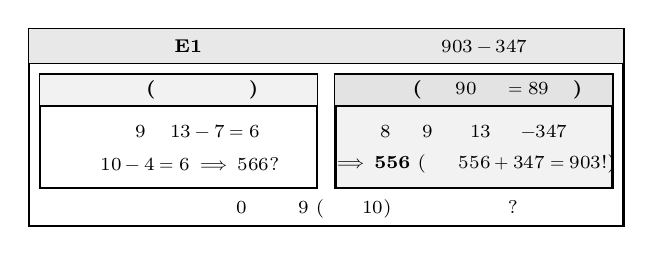
\begin{tikzpicture}[x=1cm, y=1cm, every node/.style={font=\fontsize{6.7pt}{8.6pt}\selectfont, text=black}]
  \draw[black, line width=0.9pt] (0,0) rectangle (7.55,2.50);
  \fill[gray!18] (0,2.06) rectangle (7.55,2.50);
  \draw[black, line width=0.6pt] (0,2.06) -- (7.55,2.06);
  \node at (3.775,2.28) {\textbf{បេសកកម្ម \en{E1}៖ អន្ទាក់ខ្ចីឆ្លងខ្ទង់សូន្យក្នុងប្រមាណវិធីដក $903 - 347$}};

  % Left: Student A
  \draw[black, line width=0.8pt] (0.14,0.48) rectangle (3.66,1.92);
  \fill[gray!10] (0.14,1.52) rectangle (3.66,1.92);
  \draw[black, line width=0.5pt] (0.14,1.52) -- (3.66,1.52);
  \node at (1.90,1.72) {\textbf{សិស្ស ក (ភ្លេចបន្ថយខ្ទង់ដប់)}};
  \node at (1.90,1.20) {ខ្ចីពី $9$ មក $13 - 7 = 6$};
  \node at (1.90,0.78) {ទុក $10 - 4 = 6 \implies 566$?};

  % Right: Student B
  \draw[black, line width=0.95pt, fill=gray!10] (3.89,0.48) rectangle (7.41,1.92);
  \fill[gray!22] (3.89,1.52) rectangle (7.41,1.92);
  \draw[black, line width=0.55pt] (3.89,1.52) -- (7.41,1.52);
  \node at (5.65,1.72) {\textbf{សិស្ស ខ (បំបែក $90$ ដប់ $= 89$ ដប់)}};
  \node at (5.65,1.20) {$8$ រយ \ $9$ ដប់ \ $13$ រាយ $- 347$};
  \node at (5.65,0.78) {$\implies \mathbf{556}$ (ព្រោះ $556+347=903$!)};

  \node at (3.775,0.22) {\textbf{សំណួរ៖} ហេតុអ្វីលេខ $0$ ក្លាយជា $9$ (មិនមែន $10$) ពេលខ្ចីបន្តទៅខ្ទង់រាយ?};
\end{tikzpicture}}

% ២. E2 Explore: ក្រឡាខ្ទង់នៃវិធីបូកត្រាទុក និងវិធីដកខ្ចីឆ្លងសូន្យ (ទំ.៣)
\newcommand{\figRegroupWNOneTwo}{%
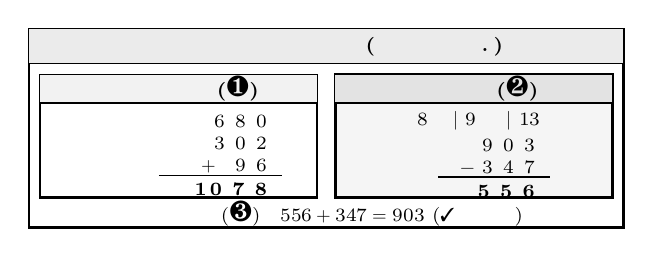
\begin{tikzpicture}[x=1cm, y=1cm, every node/.style={font=\fontsize{6.8pt}{8.8pt}\selectfont, text=black}]
  \draw[black, line width=0.9pt] (0,0) rectangle (7.55,2.52);
  \fill[gray!16] (0,2.08) rectangle (7.55,2.52);
  \draw[black, line width=0.6pt] (0,2.08) -- (7.55,2.08);
  \node at (3.775,2.30) {\textbf{ការតម្រឹមខ្ទង់ និងការខ្ចីឆ្លងខ្ទង់សូន្យ (ឧទាហរណ៍ ១ និង ៣ ទំ.៣)}};

  % Left: Addition 680 + 302 + 96
  \draw[black, line width=0.8pt] (0.14,0.38) rectangle (3.66,1.94);
  \fill[gray!10] (0.14,1.58) rectangle (3.66,1.94);
  \draw[black, line width=0.5pt] (0.14,1.58) -- (3.66,1.58);
  \node at (1.90,1.76) {\textbf{បូកតម្រឹមខ្ទង់ពីស្ដាំ (\cnum{1})}};
  \node[anchor=east] at (3.15,1.34) {$6\ \, 8\ \, 0$};
  \node[anchor=east] at (3.15,1.06) {$3\ \, 0\ \, 2$};
  \node[anchor=east] at (3.15,0.78) {$+\quad 9\ \, 6$};
  \draw[black, line width=0.6pt] (1.65,0.66) -- (3.22,0.66);
  \node[anchor=east] at (3.15,0.48) {$\mathbf{1\,0\ \, 7\ \, 8}$};

  % Right: Subtraction 903 - 347
  \draw[black, line width=0.95pt, fill=gray!8] (3.89,0.38) rectangle (7.41,1.94);
  \fill[gray!22] (3.89,1.58) rectangle (7.41,1.94);
  \draw[black, line width=0.55pt] (3.89,1.58) -- (7.41,1.58);
  \node at (5.65,1.76) {\textbf{ដកខ្ចីឆ្លងសូន្យ (\cnum{2})}};
  \node at (5.65,1.36) {\textit{ខ្ចី៖} $8$ រយ $\mid$ $9$ ដប់ $\mid$ $13$ រាយ};
  \node[anchor=east] at (6.55,1.04) {$9\ \, 0\ \, 3$};
  \node[anchor=east] at (6.55,0.76) {$-\ 3\ \, 4\ \, 7$};
  \draw[black, line width=0.6pt] (5.20,0.64) -- (6.62,0.64);
  \node[anchor=east] at (6.55,0.46) {$\mathbf{5\ \, 5\ \, 6}$};

  \node at (3.775,0.18) {ផ្ទៀងផ្ទាត់ច្រាស (\cnum{3})៖ \ $556 + 347 = 903$ (\ding{51} ត្រឹមត្រូវ)};
\end{tikzpicture}}

% % ៣. E3 Explain: គំរូរបារផ្នែក-ទាំងមូល (Part-Whole Bar Model) សម្រាប់ពូសុខ (ទំ.៣-៤)
\newcommand{\figBarModelWNOneTwo}{%
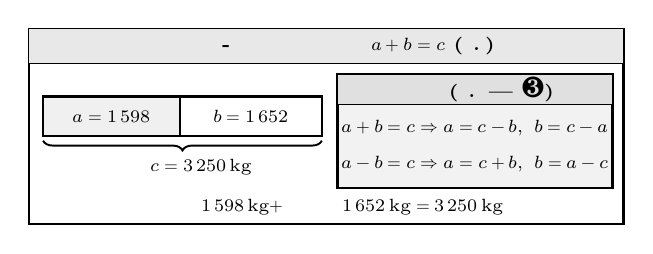
\begin{tikzpicture}[x=1cm, y=1cm, every node/.style={font=\fontsize{6.4pt}{8.4pt}\selectfont, text=black}]
  \draw[black, line width=0.9pt] (0,0) rectangle (7.55,2.48);
  \fill[gray!18] (0,2.04) rectangle (7.55,2.48);
  \draw[black, line width=0.6pt] (0,2.04) -- (7.55,2.04);
  \node at (3.775,2.26) {\textbf{គំរូរបារផ្នែក-ទាំងមូល និងទំនាក់ទំនងច្រាស $a + b = c$ (ទំ.៤)}};

  % Bar model on left
  \draw[black, line width=0.9pt, fill=gray!12] (0.18,1.12) rectangle (1.92,1.62);
  \draw[black, line width=0.9pt, fill=white] (1.92,1.12) rectangle (3.72,1.62);
  \node at (1.05,1.37) {$a = 1\,598$};
  \node at (2.82,1.37) {$b = 1\,652$};
  \draw[decorate, decoration={brace, amplitude=3.5pt, mirror}, line width=0.7pt] (0.18,1.06) -- (3.72,1.06);
  \node at (1.95,0.72) {ផលសរុប $c = 3\,250\unit{kg}$};

  % Inverse formulas box on right
  \draw[black, line width=0.9pt, fill=gray!10] (3.92,0.46) rectangle (7.41,1.90);
  \fill[gray!24] (3.92,1.52) rectangle (7.41,1.90);
  \draw[black, line width=0.55pt] (3.92,1.52) -- (7.41,1.52);
  \node at (5.665,1.71) {\textbf{វិធានទូទៅ (ទំ.៤ — \cnum{3})}};
  \node at (5.665,1.22) {$a+b=c \Rightarrow a=c-b,\ b=c-a$};
  \node at (5.665,0.76) {$a-b=c \Rightarrow a=c+b,\ b=a-c$};

  \node at (3.775,0.22) {សណ្ដែកខៀវ $1\,598\unit{kg} +$ សណ្ដែកសៀង $1\,652\unit{kg} = 3\,250\unit{kg}$};
\end{tikzpicture}}

% ៤. E4 Elaborate: តារាងភ្ញៀវទេសចរប្រាសាទអង្គរវត្ត ៣ ខែ (លំហាត់គំរូ ទំ.៤)
\newcommand{\figAngkorWNOneTwo}{%
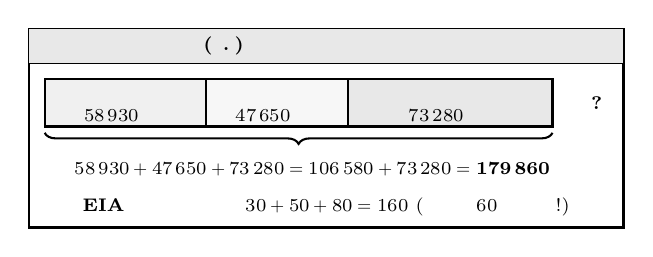
\begin{tikzpicture}[x=1cm, y=1cm, every node/.style={font=\fontsize{6.6pt}{8.6pt}\selectfont, text=black}]
  \draw[black, line width=0.9pt] (0,0) rectangle (7.55,2.52);
  \fill[gray!18] (0,2.08) rectangle (7.55,2.52);
  \draw[black, line width=0.6pt] (0,2.08) -- (7.55,2.08);
  \node at (3.775,2.30) {\textbf{លំហាត់គំរូ (ទំ.៤)៖ ភ្ញៀវទេសចរទស្សនាប្រាសាទអង្គរវត្តក្នុងរយៈពេល ៣ ខែ}};

  % Three month bars
  \draw[black, line width=0.8pt, fill=gray!12] (0.20,1.28) rectangle (2.25,1.88);
  \node at (1.225,1.70) {\textbf{ខែកុម្ភៈ}};
  \node at (1.225,1.42) {$58\,930$ នាក់};

  \draw[black, line width=0.8pt, fill=gray!6] (2.25,1.28) rectangle (4.05,1.88);
  \node at (3.15,1.70) {\textbf{ខែមីនា}};
  \node at (3.15,1.42) {$47\,650$ នាក់};

  \draw[black, line width=0.8pt, fill=gray!18] (4.05,1.28) rectangle (6.65,1.88);
  \node at (5.35,1.70) {\textbf{ខែមេសា}};
  \node at (5.35,1.42) {$73\,280$ នាក់};

  \node at (7.08,1.58) {\textbf{សរុប?}};

  \draw[decorate, decoration={brace, amplitude=4pt, mirror}, line width=0.75pt] (0.20,1.20) -- (6.65,1.20);
  \node at (3.775,0.74) {$58\,930 + 47\,650 + 73\,280 = 106\,580 + 73\,280 = \mathbf{179\,860\text{ \textbf{នាក់}}}$};
  \node at (3.775,0.26) {\textbf{\en{EIA}៖} ផ្ទៀងផ្ទាត់ខ្ទង់សិប៖ $30 + 50 + 80 = 160$ (បញ្ចប់ដោយ $60$ ត្រឹមត្រូវ!)};
\end{tikzpicture}}

% ៥. E5 Evaluate: ជម្រើសវិនិច្ឆ័យ A-D (រក x បើ x - 1408 = 2592 និង 5002 - 1645)
\newcommand{\figExitWNOneTwo}{%
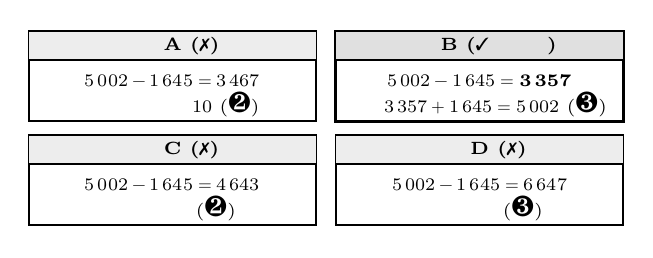
\begin{tikzpicture}[x=1cm, y=1cm, every node/.style={font=\fontsize{6.4pt}{8.4pt}\selectfont, text=black}]
  % Choice A
  \draw[black, line width=0.8pt] (0,1.32) rectangle (3.65,2.46);
  \fill[gray!14] (0,2.10) rectangle (3.65,2.46);
  \draw[black, line width=0.5pt] (0,2.10) -- (3.65,2.10);
  \node at (1.825,2.28) {\textbf{ជម្រើស \en{A} (\ding{55})}};
  \node at (1.825,1.84) {$5\,002 - 1\,645 = 3\,467$};
  \node at (1.825,1.53) {ច្រឡំទុកខ្ទង់សូន្យជា $10$ (\cnum{2})};

  % Choice B (Correct)
  \draw[black, line width=1.05pt] (3.90,1.32) rectangle (7.55,2.46);
  \fill[gray!24] (3.90,2.10) rectangle (7.55,2.46);
  \draw[black, line width=0.6pt] (3.90,2.10) -- (7.55,2.10);
  \node at (5.725,2.28) {\textbf{ជម្រើស \en{B} (\ding{51} ត្រឹមត្រូវ)}};
  \node at (5.725,1.84) {$5\,002 - 1\,645 = \mathbf{3\,357}$};
  \node at (5.725,1.53) {ព្រោះ $3\,357 + 1\,645 = 5\,002$ (\cnum{3})};

  % Choice C
  \draw[black, line width=0.8pt] (0,0) rectangle (3.65,1.14);
  \fill[gray!14] (0,0.78) rectangle (3.65,1.14);
  \draw[black, line width=0.5pt] (0,0.78) -- (3.65,0.78);
  \node at (1.825,0.96) {\textbf{ជម្រើស \en{C} (\ding{55})}};
  \node at (1.825,0.52) {$5\,002 - 1\,645 = 4\,643$};
  \node at (1.825,0.22) {ច្រឡំយកក្រោមដកលើ (\cnum{2})};

  % Choice D
  \draw[black, line width=0.8pt] (3.90,0) rectangle (7.55,1.14);
  \fill[gray!14] (3.90,0.78) rectangle (7.55,1.14);
  \draw[black, line width=0.5pt] (3.90,0.78) -- (7.55,0.78);
  \node at (5.725,0.96) {\textbf{ជម្រើស \en{D} (\ding{55})}};
  \node at (5.725,0.52) {$5\,002 - 1\,645 = 6\,647$};
  \node at (5.725,0.22) {ច្រឡំយកទៅបូកគ្នា (\cnum{3})};
\end{tikzpicture}}

\begin{document}
\fontsize{10pt}{15.2pt}\selectfont

% ============================================================================
% ក្បាលរដ្ឋបាល (Administrative Header — តាមគំរូ ls_plan.tex)
% ============================================================================
{\centering
  {\muol\fontsize{11pt}{16pt}\selectfont ព្រះរាជាណាចក្រកម្ពុជា\par}
  {\muol\fontsize{11pt}{16pt}\selectfont ជាតិ សាសនា ព្រះមហាក្សត្រ\par}
  \vspace{-3pt}{\khmflourish\par}
}

\vspace{1pt}
{\muol\fontsize{10pt}{15.5pt}\selectfont
មន្ទីរអប់រំ យុវជន និងកីឡា ខេត្តកំពង់ធំ\par
ការិយាល័យអប់រំ យុវជន និងកីឡា ស្រុកកំពង់ស្វាយ\par
អនុវិទ្យាល័យព្រះក្រសាំង\par}

\vspace{2pt}
{\centering{\muol\fontsize{11.5pt}{17pt}\selectfont កិច្ចតែងការបង្រៀន\par}}
\vspace{2pt}

% --- ព័ត៌មានទូទៅ ---
{\hspace*{2.8cm}\renewcommand{\arraystretch}{1.08}
\begin{tabular}{@{}l@{\hspace{0.35cm}}p{2.9cm}@{\hspace{0.15cm}}c@{\hspace{0.25cm}}l@{}}
  - & មុខវិជ្ជា & : & គណិតវិទ្យា ថ្នាក់ទី៧ (ពីជគណិត) \\
  - & ចំណងជើងមេរៀន & : & មេរៀនទី១៖ ចំនួនគត់ \\
  - & ចំណងជើងរង & : & ៤.១ វិធីបូកនិងវិធីដកនៃចំនួនគត់ (ទំ.៣--៤) \\
  - & រយៈពេល & : & ១ ម៉ោងសិក្សា (៥០ នាទី) \\
  - & បង្រៀនដោយ & : & ហុក ប៊ុនថែន \\
  - & កាលបរិច្ឆេទ & : & ថ្ងៃពុធ ទី៤ ខែវិច្ឆិកា ឆ្នាំ២០២៦ \\
\end{tabular}\par}

\vspace{2pt}

% --- I. វត្ថុបំណង ---
{\muol\fontsize{10pt}{15.5pt}\selectfont \enbf{I.} វត្ថុបំណង\par}
\vspace{1pt}
{\renewcommand{\arraystretch}{1.10}
\begin{tabular}{@{}p{0.55cm}@{}p{2.35cm}@{\hspace{0.15cm}}c@{\hspace{0.25cm}}p{14.95cm}@{}}
  \hfill\wcirc\hspace{0.2cm} & វិជ្ជាសម្បទា & : & សិស្សប្រាប់បានពីវិធានតម្រឹមខ្ទង់ក្នុងវិធីបូកនិងវិធីដកចំនួនគត់ ការខ្ចីឆ្លងខ្ទង់សូន្យ និងទំនាក់ទំនងច្រាសរវាងវិធីបូកនិងវិធីដក ($a+b=c \iff a=c-b, b=c-a$) បានត្រឹមត្រូវ ។ \\
  \hfill\wcirc\hspace{0.2cm} & បំណិនសម្បទា & : & សិស្សគណនាផលបូកនិងផលដកចំនួនគត់ច្រើនខ្ទង់ រកតួមិនស្គាល់ និងដោះស្រាយចំណោទជីវភាពពិត (កសិផលពូសុខ និងភ្ញៀវទេសចរប្រាសាទអង្គរវត្ត ទំ.៣--៤) លើសន្លឹកកិច្ចការបានត្រឹមត្រូវ ។ \\
  \hfill\wcirc\hspace{0.2cm} & ចរិយាសម្បទា & : & សិស្សមានទម្លាប់ផ្ទៀងផ្ទាត់លទ្ធផលគណនាដោយប្រមាណវិធីច្រាស មានភាពម៉ត់ចត់ក្នុងការរៀបខ្ទង់លេខ និងឱ្យតម្លៃលើទិន្នន័យកសិកម្មនិងទេសចរណ៍ជាតិ ។ \\
\end{tabular}\par}

\vspace{2pt}

% --- II. សម្ភារៈឧបទេស ---
{\muol\fontsize{10pt}{15.5pt}\selectfont \enbf{II.} សម្ភារៈឧបទេស\par}
\vspace{1pt}
\hspace*{0.55cm}$\bullet$\ សៀវភៅសិក្សាគោលថ្នាក់ទី៧ (ទំ.៣--៤ និងទំ.១៤) ក្ដារខៀន ដីស/ហ្វឺត បន្ទាត់ត្រង់ និង\textbf{សន្លឹកកិច្ចការសិស្សបំពេញចន្លោះ ស-ខ្មៅ} (កូដ \en{WN12} ទំព័រ ១--២ សម្រាប់សិស្ស និងទំព័រ ៣ ប្លង់ក្ដារខៀន/ចម្លើយគ្រូ — គ្មានប្រើ \en{LCD})\par

\vspace{2pt}

% --- III. វិធីសាស្រ្តបង្រៀន ---
{\muol\fontsize{10pt}{15.5pt}\selectfont \enbf{III.} វិធីសាស្រ្តបង្រៀន\par}
\vspace{1pt}
{\renewcommand{\arraystretch}{1.08}
\begin{tabular}{@{}p{0.55cm}@{}p{2.35cm}@{\hspace{0.15cm}}c@{\hspace{0.25cm}}p{14.95cm}@{}}
  \hfill$\bullet$\hspace{0.2cm} & គោលវិធី & : & សិស្សមជ្ឈមណ្ឌល (សន្លឹកកិច្ចការបំពេញចន្លោះជាគោល + ការពិភាក្សាជាក្រុមតូច ៣ នាក់) \\
  \hfill$\bullet$\hspace{0.2cm} & យុទ្ធវិធីបង្រៀន & : & គំរូស្ថាបនានិយម \en{5Es} រួមបញ្ចូល \textbf{ការបំបែកឯកតាខ្ទង់ឆ្លងសូន្យ (\en{Place-Value Decomposition})} និង \textbf{គំរូរបារផ្នែក-ទាំងមូល (\en{Part-Whole Bar Model})} \\
\end{tabular}\par}

\vspace{2pt}

% --- IV. ដំណើរការបង្រៀន ---
{\muol\fontsize{10pt}{15.5pt}\selectfont \enbf{IV.} ដំណើរការបង្រៀន\par}

{\renewcommand{\arraystretch}{1.15}
\begin{longtable}{|L{5.50cm}|L{7.90cm}|L{4.80cm}|}
\hline
\multicolumn{1}{|c|}{\cellcolor{headgray}\muol សកម្មភាពគ្រូ} &
\multicolumn{1}{c|}{\cellcolor{headgray}\muol ខ្លឹមសារមេរៀន} &
\multicolumn{1}{c|}{\cellcolor{headgray}\muol សកម្មភាពសិស្ស} \\
\hline
\endfirsthead

\hline
\multicolumn{1}{|c|}{\cellcolor{headgray}\muol សកម្មភាពគ្រូ} &
\multicolumn{1}{c|}{\cellcolor{headgray}\muol ខ្លឹមសារមេរៀន} &
\multicolumn{1}{c|}{\cellcolor{headgray}\muol សកម្មភាពសិស្ស} \\
\hline
\endhead

% ==================== ជំហានទី១ (2min) ====================
\stepheader{ជំហានទី១ \enbf{(}រដ្ឋបាលថ្នាក់\enbf{)}}
$\bullet$ ពិនិត្យវត្តមាន អនាម័យ និងសណ្ដាប់ធ្នាប់ថ្នាក់រៀន \par
$\bullet$ រៀបចំក្រុមតូច ៣ នាក់តាមតុ និងចែក\textbf{សន្លឹកកិច្ចការសិស្ស (\en{WN12} ទំព័រ ១–២)}
&
$\bullet$ រដ្ឋបាលថ្នាក់ អនាម័យ និងវិន័យសិក្សា \par
$\bullet$ ចែកសន្លឹកកិច្ចការម្នាក់ ១ សន្លឹក សម្រាប់បំពេញតាមដំណាក់កាល \en{E1--E5}
&
$\circ$ ប្រធានថ្នាក់រាយការណ៍វត្តមានសិស្ស \par
$\circ$ ទទួលសន្លឹកកិច្ចការ សរសេរឈ្មោះ និងអង្គុយតាមក្រុម ៣ នាក់ \\
\hline

% ==================== ជំហានទី២ (9min: កំណែ <=3m + រំលឹក 3m + E1 3m) ====================
\stepheader{ជំហានទី២ \enbf{(}កិច្ចការផ្ទះ \enbf{+} ទំនាក់ទំនងមេរៀនថ្មី\enbf{)}}
\ditem \textbf{កំណែកិច្ចការផ្ទះ ($\le\text{\enbf{3\,min}}$)} \par
$\bullet$ ហៅសិស្ស ២ នាក់ឡើងកែលំហាត់ទំ.១៤ លេខ ១ (ក និង ខ) លើក្ដារខៀន
&
{\centering\redsub{កំណែកិច្ចការផ្ទះមេរៀនមុន (ទំ.១៤ លេខ ១ ក និង ខ)}\par}
$\bullet$ \textbf{១ ក ($43 < n < 67$)៖} $n = 44, 45, 46, \dots, 65, 66$ (សរុប $23$ ចំនួន) \par
$\bullet$ \textbf{១ ខ (សេស $55 \le a < 65$)៖} $a = \mathbf{55, 57, 59, 61, 63}$ (យក $55$ មិនយក $65$)
&
$\circ$ ផ្ទៀងចម្លើយ និងកែតម្រូវចូលសៀវភៅកិច្ចការផ្ទះ \\[3pt]

\ditem \textbf{រំលឹកមេរៀនទាក់ទង (\enbf{3min})} \par
$\bullet$ សួរ៖ «ក្នុង $1\text{ រយ}$ មានប៉ុន្មានដប់? ចុះក្នុង $1\text{ ដប់}$ មានប៉ុន្មានរាយ?»
&
{\centering\redsub{រំលឹកទំនាក់ទំនងខ្ទង់គោល $10$}\par}
$\bullet$ $1\text{ រយ} = 10\text{ ដប់}$ និង $1\text{ ដប់} = 10\text{ រាយ}$
&
$\circ$ ឆ្លើយ៖ «$1\text{ រយ} = 10\text{ ដប់}$ ហើយ $1\text{ ដប់} = 10\text{ រាយ}$!» \\[3pt]

$\bullet$ សួរបន្ត៖ «ដូច្នេះក្នុងចំនួន $903$ បើយើងបំបែក $90\text{ ដប់}$ ឱ្យ $1\text{ ដប់}$ ទៅខ្ទង់រាយ តើសល់ប៉ុន្មានដប់ និងបានប៉ុន្មានរាយ?»
&
$\bullet$ $903 = 90\text{ ដប់} + 3\text{ រាយ} = 89\text{ ដប់} + 13\text{ រាយ}$ ($8\text{ រយ } 9\text{ ដប់ } 13\text{ រាយ}$)
&
$\circ$ ឆ្លើយ៖ «សល់ $89\text{ ដប់}$ ($8$ រយ $9$ ដប់) និងបាន $13$ រាយ!» \\[3pt]

\fiveE{E1 - Engage (3min)} \timenote{(កុំទាន់ផ្ដល់ចម្លើយ)} \par
\ditem \textbf{បេសកកម្មអន្ទាក់ខ្ចីឆ្លងខ្ទង់សូន្យ (សន្លឹកកិច្ចការ \en{E1})} \par
$\bullet$ ឱ្យសិស្សអានប្រអប់ \en{E1} ($903 - 347$) ហើយគូសជ្រើសរើសរវាង\textbf{សិស្ស ក} និង\textbf{សិស្ស ខ}
&
\redsub{បេសកកម្ម \en{E1}៖ គណនាផលដក $903 - 347$ (ឧទាហរណ៍ ៣ ទំ.៣)} \par
$\bullet$ \textbf{សិស្ស ក} គណនាឃើញ $903 - 347 = 566$ (ទុកខ្ទង់ដប់ជា $10 - 4 = 6$) \par
$\bullet$ \textbf{សិស្ស ខ} គណនាឃើញ $903 - 347 = 556$ (ខ្ទង់ដប់ក្លាយជា $9 - 4 = 5$) ។ តើអ្នកណាត្រូវ?
&
$\circ$ ពិភាក្សាជាគូ និងគូស \ding{51} ក្នុងប្រអប់ \en{E1} លើសន្លឹកកិច្ចការ \\[3pt]

&
\cfig{\figEngageWNOneTwo}
& \\
\hline

% ==================== ជំហានទី៣ (17min: E2 11m + E3 6m) ====================
\stepheader{ជំហានទី៣ \enbf{(}ខ្លឹមសារមេរៀនថ្មី\enbf{)}}
\fiveE{E2 - Explore (11min)} \par
$\bullet$ សរសេរចំណងជើងរង \textbf{៤. ប្រមាណវិធីលើចំនួនគត់} និង \textbf{៤.១ វិធីបូកនិងវិធីដកនៃចំនួនគត់} \par
\ditem \textbf{សកម្មភាព ១៖ វិធីបូកច្រើនខ្ទង់ និងចំណោទសិស្សសាលា (ទំ.៣, \enbf{5min}, \en{E2-A})} \par
$\bullet$ ឱ្យសិស្សរៀបខ្ទង់គណនាឧទាហរណ៍ ១ និងឧទាហរណ៍ ២ លើសន្លឹកកិច្ចការ \en{E2-A}
&
៤. ប្រមាណវិធីលើចំនួនគត់ \par
៤.១ វិធីបូកនិងវិធីដកនៃចំនួនគត់ \par
$\bullet$ \textbf{ឧទាហរណ៍ ១ (ទំ.៣)៖} ក. $735 + 196 = \mathbf{931}$ \quad ខ. $680 + 302 + 96 = \mathbf{1\,078}$ \par
$\bullet$ \textbf{ឧទាហរណ៍ ២ (ទំ.៣ — សិស្សទី៧ $589$, ទី៨ $546$, ទី៩ $503$)៖} សរុប $589 + 546 + 503 = \mathbf{1\,638}$ នាក់
&
$\circ$ រៀបខ្ទង់រាយក្រោមរាយ និងបូកត្រាទុកឃើញ $931, \ 1\,078$ និង $1\,638$ \\[3pt]

\ditem \textbf{សកម្មភាព ២៖ វិធីដកខ្ចីឆ្លងសូន្យ និងកសិផលពូសុខ (ទំ.៣–៤, \enbf{6min}, \en{E2-B})} \par
$\bullet$ ឱ្យសិស្សគណនាឧទាហរណ៍ ៣ ($903-347$ និង $8023-4571$) លើ \en{E2-B}
&
$\bullet$ \textbf{ឧទាហរណ៍ ៣ (ទំ.៣)៖} ក. $903 - 347 = \mathbf{556}$ \quad ខ. $8\,023 - 4\,571 = \mathbf{3\,452}$ \par
$\bullet$ \textbf{ឧទាហរណ៍ ៤ (ទំ.៣–៤ — ពូសុខប្រមូលផលសណ្ដែកសរុប $3\,250\unit{kg}$, សណ្ដែកខៀវ $1\,598\unit{kg}$)៖} \par
\hspace*{0.2cm}ម៉ាសសណ្ដែកសៀង៖ $3\,250 - 1\,598 = \mathbf{1\,652\unit{kg}}$ (ផ្ទៀង៖ $1\,598 + 1\,652 = 3\,250$)
&
$\circ$ អនុវត្តខ្ចីឆ្លងខ្ទង់សូន្យ និងផ្ទៀងផ្ទាត់ដោយបូកច្រាស \\[3pt]

&
\cfig{\figRegroupWNOneTwo}
& \\[3pt]

% --- E3 Explain (6min) ---
\fiveE{E3 - Explain (6min)} \par
$\bullet$ ដឹកនាំសិស្សទាញរក\textbf{ទំនាក់ទំនងច្រាស}រវាងវិធីបូកនិងវិធីដក (ទំ.៤) លើ \en{E3}
&
$\bullet$ \textbf{ទំនាក់ទំនងរវាងវិធីបូកនិងវិធីដក (ទំ.៤)៖} \par
\hspace*{0.15cm}១) បើ \graybox{$a + b = c$} នោះ \graybox{$a = c - b$} \ និង \ \graybox{$b = c - a$} \par
\hspace*{0.15cm}២) បើ \graybox{$a - b = c$} នោះ \graybox{$a = c + b$} \ និង \ \graybox{$b = a - c$}
&
$\circ$ បំពេញប្រអប់រូបមន្តទំនាក់ទំនងច្រាសលើ \en{E3} \\[3pt]

$\bullet$ លើកឧទាហរណ៍រហ័សអំពីការរកតួមិនស្គាល់ $x$ តាមវិធានច្រាសលើក្ដារខៀន
&
$\bullet$ \textbf{ការរកតួមិនស្គាល់តាមទំនាក់ទំនងច្រាស៖} \par
\hspace*{0.15cm}ក. បើ $x + 245 = 600$ នោះ $x = 600 - 245 = \mathbf{355}$ \par
\hspace*{0.15cm}ខ. បើ $810 - x = 275$ នោះ $x = 810 - 275 = \mathbf{535}$
&
$\circ$ អនុវត្តរកតួមិនស្គាល់ $x$ តាមវិធានច្រាស \\[3pt]

&
\cfig{\figBarModelWNOneTwo}
& \\[3pt]

$\bullet$ ភ្ជាប់\textbf{ធនាគារហេតុផល \cnum{1}} និង \textbf{\cnum{2}} លើក្ដារខៀន និងសន្លឹកកិច្ចការ
&
\textbf{ធនាគារហេតុផល (\en{Warrant Bank})៖} \par
\cnum{1} \textbf{តម្រឹមខ្ទង់៖} រៀបខ្ទង់រាយក្រោមរាយ ដប់ក្រោមដប់ រយក្រោមរយពីស្ដាំទៅឆ្វេង
&
$\circ$ ផ្ទៀងលេខកូដ \cnum{1} លើសន្លឹកកិច្ចការ \\[3pt]

$\bullet$ សង្កត់ធ្ងន់លើការបំបែកខ្ទង់សូន្យក្នុងលេខកូដ \cnum{2}
&
\cnum{2} \textbf{ខ្ចីឆ្លងសូន្យ៖} បំបែក $1\text{ រយ} = 9\text{ ដប់} + 10\text{ រាយ}$ (លេខ $0$ កណ្ដាលក្លាយជា $9$ មិនមែន $10$)
&
$\circ$ ផ្ទៀងលេខកូដ \cnum{2} លើសន្លឹកកិច្ចការ \\[3pt]

$\bullet$ ភ្ជាប់\textbf{ធនាគារហេតុផល \cnum{3}--\cnum{4}} សម្រាប់ផ្ទៀងផ្ទាត់ច្រាស និងចំណោទ
&
\cnum{3} \textbf{ផ្ទៀងផ្ទាត់ច្រាស៖} $a - b = c \iff c + b = a$ (ប្រើវិធីបូកត្រួតពិនិត្យផលដកជានិច្ច) \par
\cnum{4} \textbf{របារផ្នែក-ទាំងមូល៖} ផ្នែកនៅសល់ $=$ ចំនួនសរុប $-$ ផ្នែកដែលស្គាល់
&
$\circ$ ផ្ទៀងលេខកូដ \cnum{3}--\cnum{4} លើសន្លឹកកិច្ចការ \\
\hline

% ==================== ជំហានទី៤ (20min: E4 10m + E5 10m) ====================
\stepheader{ជំហានទី៤ \enbf{(}ពង្រីកចំណេះដឹង\enbf{)}}
\fiveE{E4 - Elaborate (10min)} \par
\ditem \textbf{លំហាត់គំរូ៖ ភ្ញៀវទេសចរទស្សនាប្រាសាទអង្គរវត្ត ៣ ខែ (ទំ.៤)} \par
$\bullet$ ឱ្យសិស្សអានតារាងទិន្នន័យភ្ញៀវទេសចរទាំង ៣ ខែលើ \en{E4}
&
{\muol លំហាត់គំរូ} \textbf{(ទំ.៤ — ភ្ញៀវទេសចរអន្តរជាតិទិញសំបុត្រចូលទស្សនាប្រាសាទអង្គរវត្ត)៖} \par
$\bullet$ ខែកុម្ភៈមាន $58\,930$ នាក់, ខែមីនាមាន $47\,650$ នាក់, និងខែមេសាមាន $73\,280$ នាក់
&
$\circ$ កំណត់ទិន្នន័យភ្ញៀវតាមខែនីមួយៗលើ \en{E4} \\[3pt]

$\bullet$ ណែនាំឱ្យបូកជា ២ ជំហានដោយតម្រឹមខ្ទង់ពីស្ដាំ (\cnum{1})
&
$\bullet$ ជំហានទី ១ (បូកខែកុម្ភៈនិងមីនា)៖ $58\,930 + 47\,650 = \mathbf{106\,580}$ នាក់ \par
$\bullet$ ជំហានទី ២ (បូកសរុបទាំង ៣ ខែ)៖ $106\,580 + 73\,280 = \graybox{$179\,860\text{ នាក់}$}$
&
$\circ$ រៀបខ្ទង់បូកជា ២ ជំហាន ឃើញសរុប $179\,860$ នាក់ \\[3pt]

&
\cfig{\figAngkorWNOneTwo}
& \\[3pt]

$\bullet$ សួរសំណួរឆ្លុះបញ្ចាំង \textbf{\en{EIA Looking-Back} (1min)}
&
\textbf{\en{EIA Looking-Back}៖} «តើខែមេសាមានភ្ញៀវច្រើនជាងខែមីនាប៉ុន្មាននាក់? យើងត្រូវប្រើប្រមាណវិធីអ្វី?» ($\to$ វិធីដក៖ $73\,280 - 47\,650 = \mathbf{25\,630}$ នាក់!)
&
$\circ$ គណនាផលសងរវាងខែមេសានិងខែមីនាឃើញ $25\,630$ នាក់ \\[3pt]

% --- E5 Evaluate (10min) ---
\fiveE{E5 - Evaluate (10min)} \par
\ditem \textbf{ប្រតិបត្តិជាក្រុមតូច ៣ នាក់ (4min, សន្លឹកកិច្ចការ \en{E5})} \par
$\bullet$ ឱ្យសិស្សគណនាលំហាត់ប្រតិបត្តិ ក (ទំ.៤) ជាក្រុម
&
{\muol លំហាត់ប្រតិបត្តិ} \textbf{(សៀវភៅគោល ទំ.៤)៖} \par
$\bullet$ \textbf{ក.} $46\,382 + 6\,948 + 164\,968 + 1\,896 = 53\,330 + 166\,864 = \graybox{$220\,194$}$
&
$\circ$ រៀបខ្ទង់បូកជាគូៗ ឃើញ $220\,194$ \\[3pt]

$\bullet$ ឱ្យសិស្សគណនាលំហាត់ប្រតិបត្តិ ខ (ទំ.៤) តាមលំដាប់ពីឆ្វេងទៅស្ដាំ
&
$\bullet$ \textbf{ខ.} $1\,712\,366 - 492\,135 - 54\,201 = 1\,220\,231 - 54\,201 = \graybox{$1\,166\,030$}$
&
$\circ$ ដកតាមលំដាប់ពីឆ្វេងទៅស្ដាំឃើញ $1\,166\,030$ \\[3pt]

$\bullet$ ឱ្យក្រុមសិស្សផ្ទៀងផ្ទាត់និង\textbf{បិទបេសកកម្ម \en{E1} (2min)}
&
$\bullet$ \textbf{បិទបេសកកម្ម \en{E1}៖} \textbf{សិស្ស ខ} ត្រឹមត្រូវ! $903 - 347 = \mathbf{556}$ ព្រោះ $556 + 347 = 903$ (\cnum{2}, \cnum{3}) ឯ $566 + 347 = 913 \ne 903$!
&
$\circ$ បិទបេសកកម្ម \en{E1} ឃើញសិស្ស ខ ត្រឹមត្រូវ ($556$) \\[3pt]

\ditem \textbf{សំណួរវិនិច្ឆ័យ \en{A--D} និងសំបុត្រចេញ (4min)} \par
$\bullet$ សរសេរលំហាត់វិនិច្ឆ័យ $5\,002 - 1\,645$ និងជម្រើស \en{A--D} លើក្ដារខៀន
&
{\centering\textbf{សំណួរវិនិច្ឆ័យ \en{A--D}៖ តើផលដកឆ្លងសូន្យពីរខ្ទង់ $5\,002 - 1\,645$ ស្មើនឹងប៉ុន្មាន?}\par}
&
$\circ$ អានប្រធានលំហាត់ និងសាកល្បងបំបែក $5\,002 = 4\text{ ពាន់ } 9\text{ រយ } 9\text{ ដប់ } 12\text{ រាយ}$ \\[3pt]

$\bullet$ ឱ្យសិស្សគូសរង្វង់ជម្រើសត្រូវលើសន្លឹកកិច្ចការ រួចលើកម្រាមដៃ ១--៤ ព្រមគ្នា
&
$\bullet$ ផ្ទៀងកំហុសក្នុងជម្រើសនីមួយៗតាមលេខកូដហេតុផល \cnum{2} (ខ្ចីឆ្លងសូន្យ) និង \cnum{3} (បូកច្រាស)
&
$\circ$ វិភាគជម្រើស \en{A--D} និងលើកម្រាមដៃ ២ (\textbf{ជម្រើស \en{B}}) \\[3pt]

&
\cfig{\figExitWNOneTwo}
& \\[3pt]

$\bullet$ បញ្ជាក់ចម្លើយត្រូវ (\textbf{ជម្រើស \en{B}}) និងឱ្យបំពេញ\textbf{សំបុត្រចេញ ៦០ វិនាទី}
&
$\bullet$ \textbf{សំបុត្រចេញ៖} បើ $x - 1\,408 = 2\,592$ នោះ $x = 2\,592 + 1\,408 = \mathbf{4\,000}$ (\cnum{3}) ។
&
$\circ$ បំពេញសំបុត្រចេញលើសន្លឹកកិច្ចការមុនបញ្ចប់ម៉ោង \\
\hline

% ==================== ជំហានទី៥ (<=2min) ====================
\stepheader{ជំហានទី៥ \enbf{(}កិច្ចការផ្ទះ \enbf{+} បណ្ដាំផ្ញើ\enbf{)}}
\timenote{ចំណាយពេលឱ្យតិចបំផុតកុំឱ្យលើស 2min} \par
$\bullet$ ណែនាំប្រអប់\textbf{កិច្ចការផ្ទះ}លើសន្លឹកកិច្ចការទំព័រ ២ (លំហាត់ទំ.១៤ លេខ ៣)
&
{\centering{\muol កិច្ចការផ្ទះ} \textbf{(សៀវភៅគោល ទំ.១៤ លេខ ៣)}\par} \par
$\bullet$ \textbf{លេខ ៣៖} នៅអនុវិទ្យាល័យមួយមានសិស្សប្រុស $679$ នាក់និងសិស្សស្រី $578$ នាក់ ។ ក្នុងមួយឆ្នាំសិស្សដែលអានសៀវភៅនៅក្នុងបណ្ណាល័យបាន $4$ ក្បាល ឬច្រើនជាង $4$ ក្បាល មានចំនួន $824$ នាក់ ។ តើសិស្សដែលបានអានសៀវភៅតិចជាង $4$ ក្បាលមានប៉ុន្មាននាក់?
&
$\circ$ គូសចំណាំលំហាត់លេខ ៣ ទំ.១៤ \\[3pt]

$\bullet$ ផ្ដាំផ្ញើឱ្យផ្ទៀងផ្ទាត់ចម្លើយកិច្ចការផ្ទះ និងអានមុនចំណុច ៤.២ (ទំ.៤–៦)
&
$\bullet$ \textbf{បណ្ដាំផ្ញើ៖} ប្រើវិធីបូកផ្ទៀងផ្ទាត់ចម្លើយកិច្ចការផ្ទះ និងអានមុន \textbf{៤.២ វិធីគុណនិងវិធីចែកចំនួនគត់} (ទំ.៤–៦) ។
&
$\circ$ កត់ត្រាបណ្ដាំផ្ញើ ទុកសន្លឹកកិច្ចការក្នុងសៀវភៅ និងជម្រាបលាគ្រូ \\
\hline
\end{longtable}}

\vspace{6pt}
% --- ហត្ថលេខា (កាលបរិច្ឆេទត្រូវគ្នា ១០០% នឹងខាងលើ) ---
{\centering
\hspace*{5.2cm}\begin{minipage}{11.5cm}
  \centering
  ថ្ងៃពុធ ៩រោច ខែអស្សុជ ឆ្នាំមមី អដ្ឋស័ក ពុទ្ធសករាជ ២៥៧០\par
  កំពង់ស្វាយ, ថ្ងៃទី៤ ខែវិច្ឆិកា ឆ្នាំ២០២៦\par
  \vspace{2pt}
  {\muol គ្រូបង្រៀន\par}
  \vspace{32pt}
  \hfill{\muol ហុក ប៊ុនថែន}\hspace*{1.4cm}
\end{minipage}\par}

\end{document}
